\documentclass{ctexart}
\usepackage{tikz}
\usepackage{t-angles}
\usepackage{amssymb}
\usepackage{tikz} 
\usepackage[mathscr]{eucal}

\usepackage{tikz}
\usepackage{pgfplots}
\usetikzlibrary{quotes,angles}
\usetikzlibrary{calc}
\usetikzlibrary{decorations.pathreplacing}

\makeatletter
\newcommand{\rmnum}[1]{\romannumeral #1}
\newcommand{\Rmnum}[1]{\expandafter\@slowromancap\romannumeral #1@}
\makeatother

\begin{document}
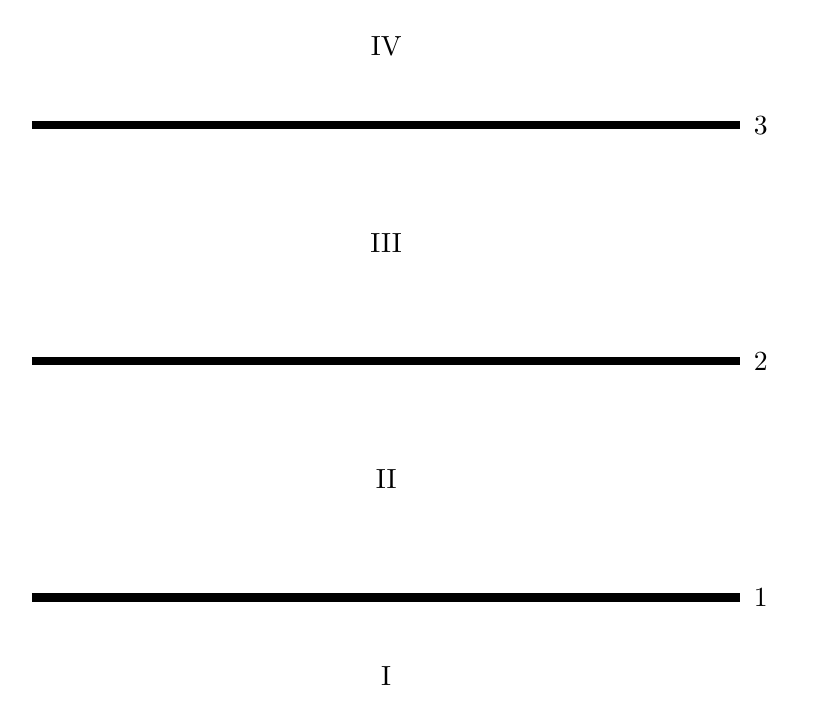
\begin{tikzpicture}
    \node at(4.5,2) {\Rmnum{1}};
    \draw [line width =3pt] (0,3)--(9,3) node[right] {1};
    
    \node at(4.5,4.5) {\Rmnum{2}};
    \draw [line width =3pt] (0,6)--(9,6) node[right] {2};
    
    \node at(4.5,7.5) {\Rmnum{3}};
    \draw [line width =3pt] (0,9)--(9,9) node[right] {3};
    
    \node at(4.5,10) {\Rmnum{4}};
\end{tikzpicture}

\begin{tikzpicture}
    \draw[->] (0,0) --(6,0) node[right] {$r$};
    \draw[->] (0,0) --(0,3) node[above] {$E$};
    \draw[loosely dashed] (0.5,3) --(0.5,0) node[below] {$R$};
    \draw[loosely dashed] (0.5,2) --(0,2) node[left] {$\frac{\lambda}{2\pi\varepsilon_0R}$};
    \draw (0.5,2) circle (.1);
    \filldraw (0.5,1) circle (.1);
    \draw[loosely dashed] (0.5,1) --(0,1) node[left] {$\frac{\lambda}{4\pi\varepsilon_0R}$};
    \draw[domain =0.5:5] plot (\x ,{1/\x}) ;
    \end{tikzpicture}


\begin{tikzpicture}
    \draw (0,0) --(0,5) node[above] {+};
    \draw (2,0) --(2,5) node[above] {-};
    \draw[->] (-3,2.5) --(5,2.5) node[right] {$x$};
    \filldraw (1,2.5) circle (.1) node[below] {0};
\end{tikzpicture}

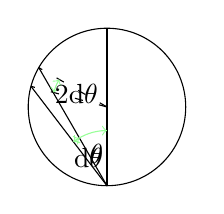
\begin{tikzpicture}
    \draw (1,1) circle (1);
    \draw (1,0) --(1,2);
    \draw (1,0) --(0.035,1.2622);
    \draw (1,0) --(0.1339,1.4998);
    \draw[loosely dashed] (1,1) --(0.035,1.2622);
    \draw[loosely dashed] (1,1) --(0.1339,1.4998);
    \coordinate (o) at (1,1);
    \coordinate (a) at (0.035,1.2622);
    \coordinate (b) at (0.1339,1.4998);
    \coordinate (p) at (1,0);
    \coordinate (c) at (1,2);
    \pic["$2\mathrm{d}\theta$", draw=green!40, <->, angle eccentricity=0.6, angle radius=0.7cm]
    {angle=b--o--a};
    \pic["$\mathrm{d}\theta$", draw=green!40, <->, angle eccentricity=0.6, angle radius=0.7cm]
    {angle=b--p--a};
    \pic["$\theta$", draw=green!40, <->, angle eccentricity=0.6, angle radius=0.7cm]
    {angle=c--p--a};
\end{tikzpicture}

\begin{tikzpicture}
    \coordinate (o) at (5,5);
    \coordinate (a) at (0.175,6.311);
    \coordinate (b) at (0.6695,7.499);
    \coordinate (p) at (5,0);
    \coordinate (c) at (5,10);
    \draw (o) circle (5);
    \draw (p) --(c);
    \draw (p) --(a);
    \draw (b) --(p) node[below] {$P$};
    \draw[loosely dashed] (o) --(a) ;
    \draw[loosely dashed] (o) --(b);
    
    \pic["$2\mathrm{d}\theta$", draw=green!40, <->, angle eccentricity=0.6, angle radius=0.7cm]
    {angle=b--o--a};
    \pic["$\mathrm{d}\theta$", draw=green!40, <->, angle eccentricity=0.9, angle radius=1cm]
    {angle=b--p--a};
    \pic["$\theta$", draw=green!40, <->, angle eccentricity=1.05, angle radius=5cm]
    {angle=c--p--a};
\end{tikzpicture}

\begin{tikzpicture}
    \draw[->] (-5,0) --(5,0) node[right]{$x$};
    \draw[->] (0,-5) --(0,5) node[right]{$E$};
    \draw[loosely dashed] (-1,5) --(-1,0)node[below]{$-\frac{d}{2}$};
    \draw[loosely dashed] (1,5) --(1,0)node[below]{$\frac{d}{2}$};
    \draw (-1,3) --(1,3);
    \node at(0.3,3) {$\frac{\sigma_e}{\varepsilon_0}$};
\end{tikzpicture}

\begin{tikzpicture}
    \draw[->] (-5,0) --(5,0) node[right]{$x$};
    \draw[->] (0,-5) --(0,5) node[right]{$U$};
    \draw[loosely dashed] (-1,5) --(-1,0)node[below]{$-\frac{d}{2}$};
    \draw[loosely dashed] (1,5) --(1,0)node[below]{$\frac{d}{2}$};
    \draw[loosely dashed] (-1,0) --(-1,-5);
    \draw[loosely dashed] (1,0) --(1,-5);
    \draw (-1,-3) --(1,3);
    \draw[loosely dashed] (1,3) --(0,3)node[left]{$\frac{\sigma_e d}{2\varepsilon_0}$};
    
\end{tikzpicture}

\begin{tikzpicture}
    \coordinate (p) at (3,4);
    \coordinate (o) at (0,0);
    \coordinate (a) at (1,0);
    \coordinate (b) at (-1,0);
    \draw[->] (-5,0) --(5,0) node[right]{$x$};
    \draw[->] (0,-5) --(0,5) node[right]{$y$};
    \draw[->] (1,0) --(1,-1) node[below]{$\vec{p}_1$};
    \draw[->] (-1,0) --(-1,1) node[above]{$\vec{p}_2$};
    \draw[->] (o) --(p) node[right]{$P(r,\theta)$};
    \draw[->] (a) --(p) ;
    \draw[->] (b) --(p) ;
    \node at(2,1) {$\vec{r}_1$};
    \node at(1,2.5) {$\vec{r}_2$};
    \pic["$\theta$", draw=red!40, <->, angle eccentricity=0.6, angle radius=0.7cm]
    {angle=a--o--p};
\end{tikzpicture}
$\mathscr{E}$



    \begin{tikzpicture}
        \draw (-2,5) --(-2,-5) node[below]{1};
        \draw (-1,5) --(-1,-5) node[below]{2};
        \draw (1,5) --(1,-5) node[below]{3};
        \draw (3,5) --(3,-5) node[below]{4};
        \draw (-1.5,4) rectangle (2,3);
        \draw (-1.5,-4) rectangle (-3,-3);
        \draw (2,-4) rectangle (4,-3);
        \node at(0,3.5){\Rmnum{1}};
        \node at(-2.5,-3.5){\Rmnum{2}};
        \node at(3.5,-3.5){\Rmnum{3}};
    \end{tikzpicture}
    
    \begin{tikzpicture}
        \draw[->] (-5,0) --(5,0) node[right]{$x$};
        \draw[->] (0,-5) --(0,5) node[right]{$y$};
        \filldraw (1,1) circle (.1)node[right]{B};
        \filldraw (-1,1) circle (.1)node[left]{A};
        \filldraw (1,-1) circle (.1)node[right]{C};
        \filldraw (-1,-1) circle (.1)node[left]{D};
    \end{tikzpicture}

    \begin{tikzpicture}
        
        \coordinate (a) at (1,0);
        \coordinate (b) at (-1,0);
        \draw[->] (-5,0) --(5,0) node[right]{$x$};
        \draw[->] (0,-5) --(0,5) node[right]{$y$};
        \filldraw (a) circle (.1)node[right]{$\lambda$};
        \filldraw (b) circle (.1)node[right]{$-\lambda$};
    \end{tikzpicture}

    \begin{tikzpicture}
        
        \draw (-5,5) rectangle (5,4.9);
        \draw (-5,4.9) rectangle (5,3);
        \draw (-5,3) rectangle (5,0);
        \draw (-5,0) rectangle (5,-0.1);
        \node at(0,3.5){$\varepsilon_1$};
        \node at(0,1.5){$\varepsilon_2$};
        \draw (-1,4.95) rectangle (1,4);
        \draw (-1,-0.05) rectangle (1,1);
        \node at(0,4.5){$\Rmnum{1}$};
        \node at(0,0.5){$\Rmnum{2}$};
    \end{tikzpicture}

    \begin{tikzpicture}
        \coordinate (a) at (1,0);
        \coordinate (b) at (1.8,2.4);
        \coordinate (o) at (0,0);
        \draw[->] (-3,0) --(5,0)node[right]{$P$};
        \draw (0,0) circle (3);
        \draw[->] (0,0) --(1.8,2.4);
        \pic["$\theta$", draw=green!40, <->, angle eccentricity=0.6, angle radius=0.7cm]
    {angle=a--o--b};
    \end{tikzpicture}

    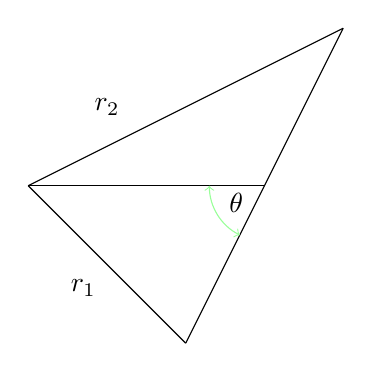
\begin{tikzpicture}
        \coordinate (a) at (3,0);
        \coordinate (b) at (4,2);
        \coordinate (o) at (0,0);
        \coordinate (c) at (2,-2);
        \draw (o) --(a);
        \draw (o) --(b);
        \draw (o) --(c);
        \draw (b) --(c);
        \node at(0.7,-1.3) {$r_1$};
        \node at(1,1) {$r_2$};
        \pic["$\theta$", draw=green!40, <->, angle eccentricity=0.6, angle radius=0.7cm]
    {angle=o--a--c};
    \end{tikzpicture}
\end{document}
